% begin module cardioid-tangents-ex9
\begin{frame}
\begin{example} %[Example 9, p. 681]
Find the points on \alert<handout:0| 3-6>{$r = 1+\sin\theta$} where the tangent is horizontal or vertical.
\begin{columns}[c]
\column{.4\textwidth}
\psset{xunit=1.2cm, yunit=1.2cm}
\begin{pspicture}(-2.2, -0.900000)(2.2,2.6)
\tiny
\fcAxesStandard{-2.1}{-0.650000}{2.1}{2.4}
%Calculator command: drawPolar{}(\sin{}t+1, 0, 2 \pi)
\parametricplot[linecolor=\fcColorGraph, plotpoints=1000, algebraic=false]{0}{6.28319}{1.0000000 t 57.29578 mul sin add t 57.29578 mul cos mul 1.0000000 t 57.29578 mul sin add t 57.29578 mul sin mul }

\uncover<15->{%
\fcFullDotBlue{1.299038}{0.75}
\psline[linecolor=\fcColorTangent](1.299038,0.35)(1.299038,1.15)
\rput[l](1.35, 0.75){$\left(\frac{3}{2},\frac{\pi}{6}\right)$}
}%
\uncover<14->{%
\fcFullDotBlue{0}{2}
\psline[linecolor=\fcColorTangent](-0.4,2)(0.4,2)
\rput[bl](0.05,2.05){$\left(2,\frac{\pi}{2}\right)$}
}%
\uncover<15->{%
\fcFullDotBlue{-1.299038}{0.75}
\psline[linecolor=\fcColorTangent](-1.299038,0.35)(-1.299038,1.15)
\rput[r](-1.35,0.75){$\left(\frac{3}{2},\frac{5\pi}{6}\right)$}
}%
\uncover<14->{%
\fcFullDotBlue{-0.433013}{-0.25}
\psline[linecolor=\fcColorTangent](-0.033013,-0.25)(-0.833013,-0.25)
\rput[t](-0.433013,-0.3){$\left(\frac{1}{2},\frac{7\pi}{6}\right)$}
}
\uncover<22->{%
\fcFullDotBlue{0}{0}
\psline[linecolor=\fcColorTangent](0,-0.4)(0,0.4)
\rput[bl](0.05,0.05){$\left(0,\frac{3\pi}{2}\right)$}
}%
\uncover<14->{%
\fcFullDotBlue{0.433013}{-0.25}
\psline[linecolor=\fcColorTangent](0.033013,-0.25)(0.833013,-0.25)
\rput[t](0.433013,-0.3){$\left(\frac{1}{2},\frac{11\pi}{6}\right)$}
}%
\end{pspicture}

%\ \only<handout:0| -13>{%
%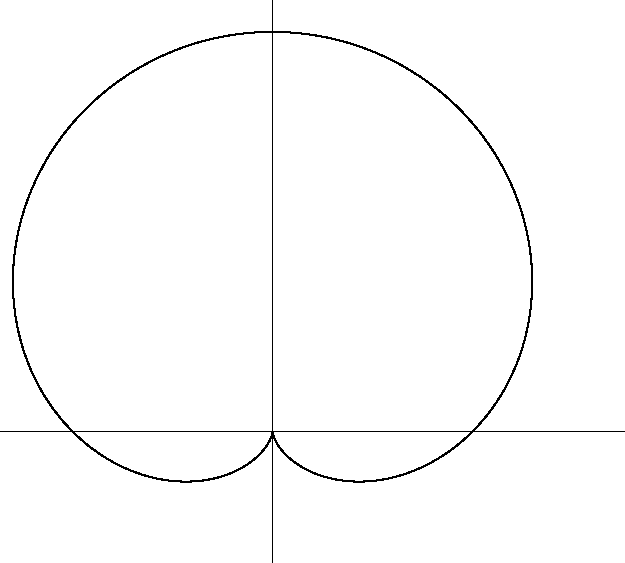
\includegraphics[height=4cm]{polar-curves/pictures/11-03-tangenta.pdf}%
%}%
%\only<handout:0| 14>{%
%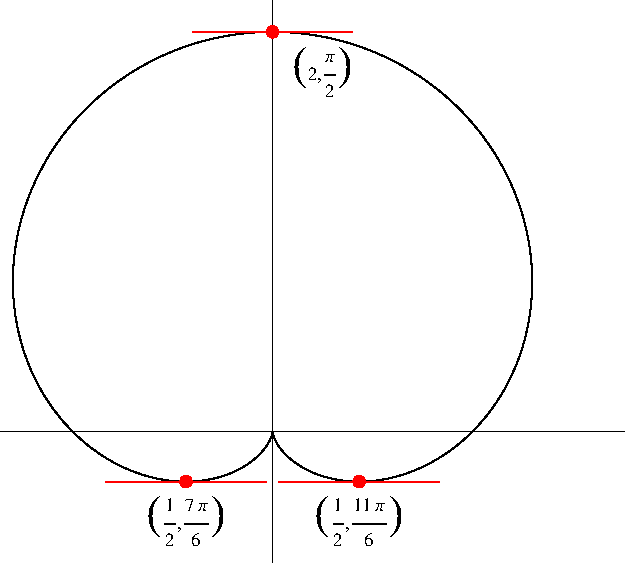
\includegraphics[height=4cm]{polar-curves/pictures/11-03-tangentb.pdf}%
%}%
%\only<handout:0| 15>{%
%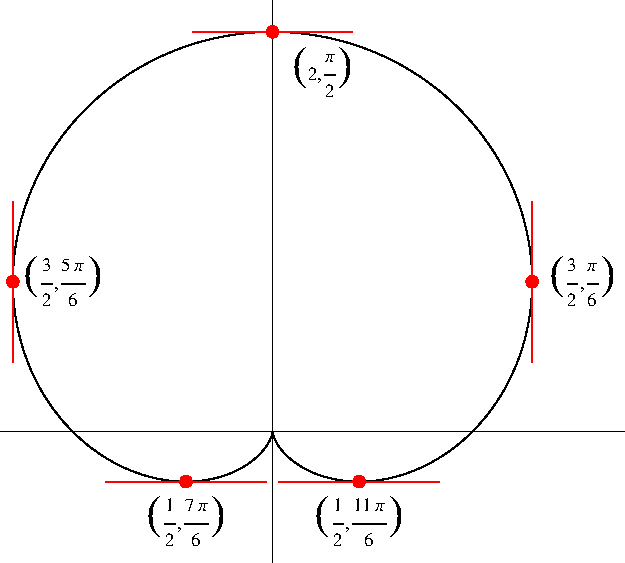
\includegraphics[height=4cm]{polar-curves/pictures/11-03-tangentc.pdf}%
%}%
%\only<handout:0| 16-21>{%
%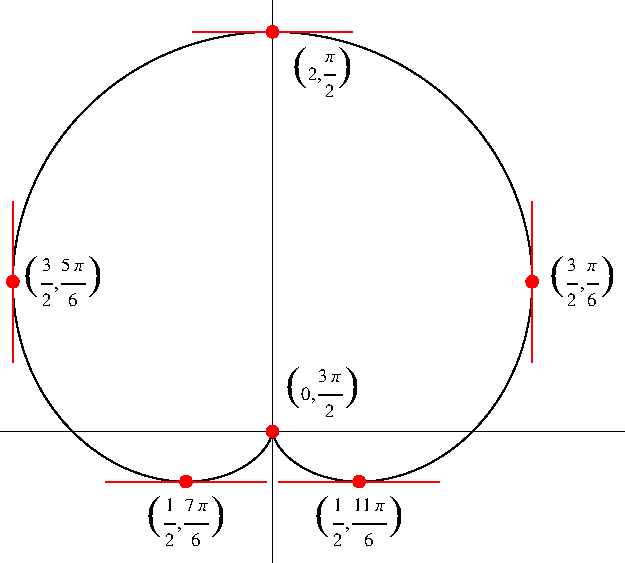
\includegraphics[height=4cm]{polar-curves/pictures/11-03-tangentd.pdf}%
%}%
%\only<22->{%
%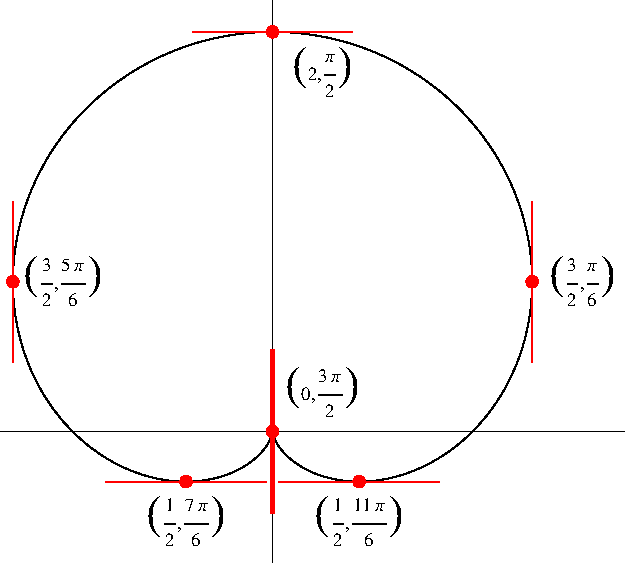
\includegraphics[height=4cm]{polar-curves/pictures/11-03-tangente.pdf}%
%}%
\column{.62\textwidth}
\abovedisplayskip=0pt
\belowdisplayskip=0pt
\[
\begin{array}{r@{\ }c@{\ }l}
\uncover<2->{%
\frac{\diff y}{\diff x} %
}%
&\uncover<2->{ = } & %
\uncover<2->{\frac{\alert<handout:0| 5-6>{\frac{\diff r}{\diff\theta}}\sin \theta + \alert<handout:0| 3-4>{r}\cos \theta}{\alert<handout:0| 5-6>{\frac{\diff r}{\diff \theta}}\cos \theta - \alert<handout:0| 3-4>{r}\sin \theta}}%
\uncover<3->{ = \frac{\uncover<6->{\alert<handout:0| 6>{\cos\theta }}\sin\theta + \uncover<4->{\alert<handout:0| 4>{(1+\sin\theta )}}\cos\theta}{\uncover<6->{\alert<handout:0| 6>{\cos\theta }}\cos \theta - \uncover<4->{\alert<handout:0| 4>{(1+\sin \theta )}}\sin\theta}}\\%
&\uncover<7->{ = } & %
\uncover<7->{\frac{\cos\theta (1+2\sin \theta )}{1 - 2\sin^2\theta - \sin\theta}}%
\uncover<8->{ = \frac{\cos\theta (1+2\sin\theta)}{(1+\sin\theta )(1-2\sin\theta )}}%
\end{array}
\]
\begin{itemize}
\item<9->  $\cos\theta (1+2\sin \theta ) = 0$ \\
 when \alert<handout:0| 10-11>{$\theta =$ \uncover<11->{$\alert<handout:0| 14>{\frac{\pi}{2}}, \alert<handout:0| 16>{\frac{3\pi}{2}}, \alert<handout:0| 14>{\frac{7\pi}{6}}, \alert<handout:0| 14>{\frac{11\pi}{6}}$.}}%
\item<9->  $(1+\sin \theta ) (1-2\sin \theta ) = 0$ \\
 when \alert<handout:0| 12-13>{$\theta = $ \uncover<13->{$\alert<handout:0| 16>{\frac{3\pi}{2}}, \alert<handout:0| 15>{\frac{\pi}{6}}, \alert<handout:0| 15>{\frac{5\pi}{6}}$.}}%
\end{itemize}
\end{columns}
\begin{itemize}
\item<14->  Horizontal tangents at $(2,\alert<handout:0| 14>{\pi /2})$, $(1/2, \alert<handout:0| 14>{7\pi /6})$, and $(1/2, \alert<handout:0| 14>{11\pi /6})$.
\item<15->  Vertical tangents at $(3/2,\alert<handout:0| 15>{\pi /6})$, and $(3/2, \alert<handout:0| 15>{5\pi /6})$.
\item<16->  If \alert<handout:0| 16>{$\theta = 3\pi /2$}, top and bottom are both $0$, so \alert<handout:0| 20-21>{use L'Hospital's Rule}.
\end{itemize}
\abovedisplayskip=0pt
\belowdisplayskip=0pt
\[
\begin{array}{l}
\uncover<17->{{\displaystyle \lim_{\theta\to 3\pi/2^-}}\frac{\diff y}{\diff x} = }%
\uncover<17->{ \alert<handout:0| 18-19>{{\displaystyle \lim_{\theta\to 3\pi/2^-}}\frac{1+2\sin\theta}{1-2\sin\theta}}\cdot %
 \alert<handout:0| 20-21>{{\displaystyle \lim_{\theta\to 3\pi/2^-}}\frac{\cos\theta}{1+\sin\theta}} }%
\uncover<18->{=} \uncover<19->{\alert<handout:0| 19>{-\frac{1}{3}}} \uncover<21->{\alert<handout:0| 21>{{\displaystyle \lim_{\theta\to 3\pi/2^-}}\frac{-\sin\theta}{\cos\theta}}} %
\uncover<22->{= \infty}
\end{array}
\]
\end{example}
\end{frame}
% end module cardioid-tangents-ex9
